\chapter{Neural Optimal Transport}
\label{cha:cellot}


\dictum[Gottfried Wilhelm Leibniz, \textit{Nouveaux essais sur l'entendement humain} (1765)]{%
  Tout va par degr\'e dans la nature, et rien par saut, et cette regle \`a l'\'egard des changements est une partie de ma loi de la continuit\'e.}%
\vskip 1em

\verpar{Contributions}{
Most of the material in this chapter has been already published in the following journal article:
\begin{itemize}
	\item[] Charlotte Bunne, Stefan G Stark, Gabriele Gut, Jacobo Sarabia del Castillo, Kjong-Van Lehmann, Lucas Pelkmans, Andreas Krause, and Gunnar R{\"a}tsch. Learning Single-Cell Perturbation Responses using Neural Optimal Transport. \textit{Nature Methods}, 2023.
	\vspace{-9pt}
\end{itemize}
}

\begin{figure}
    \centering
    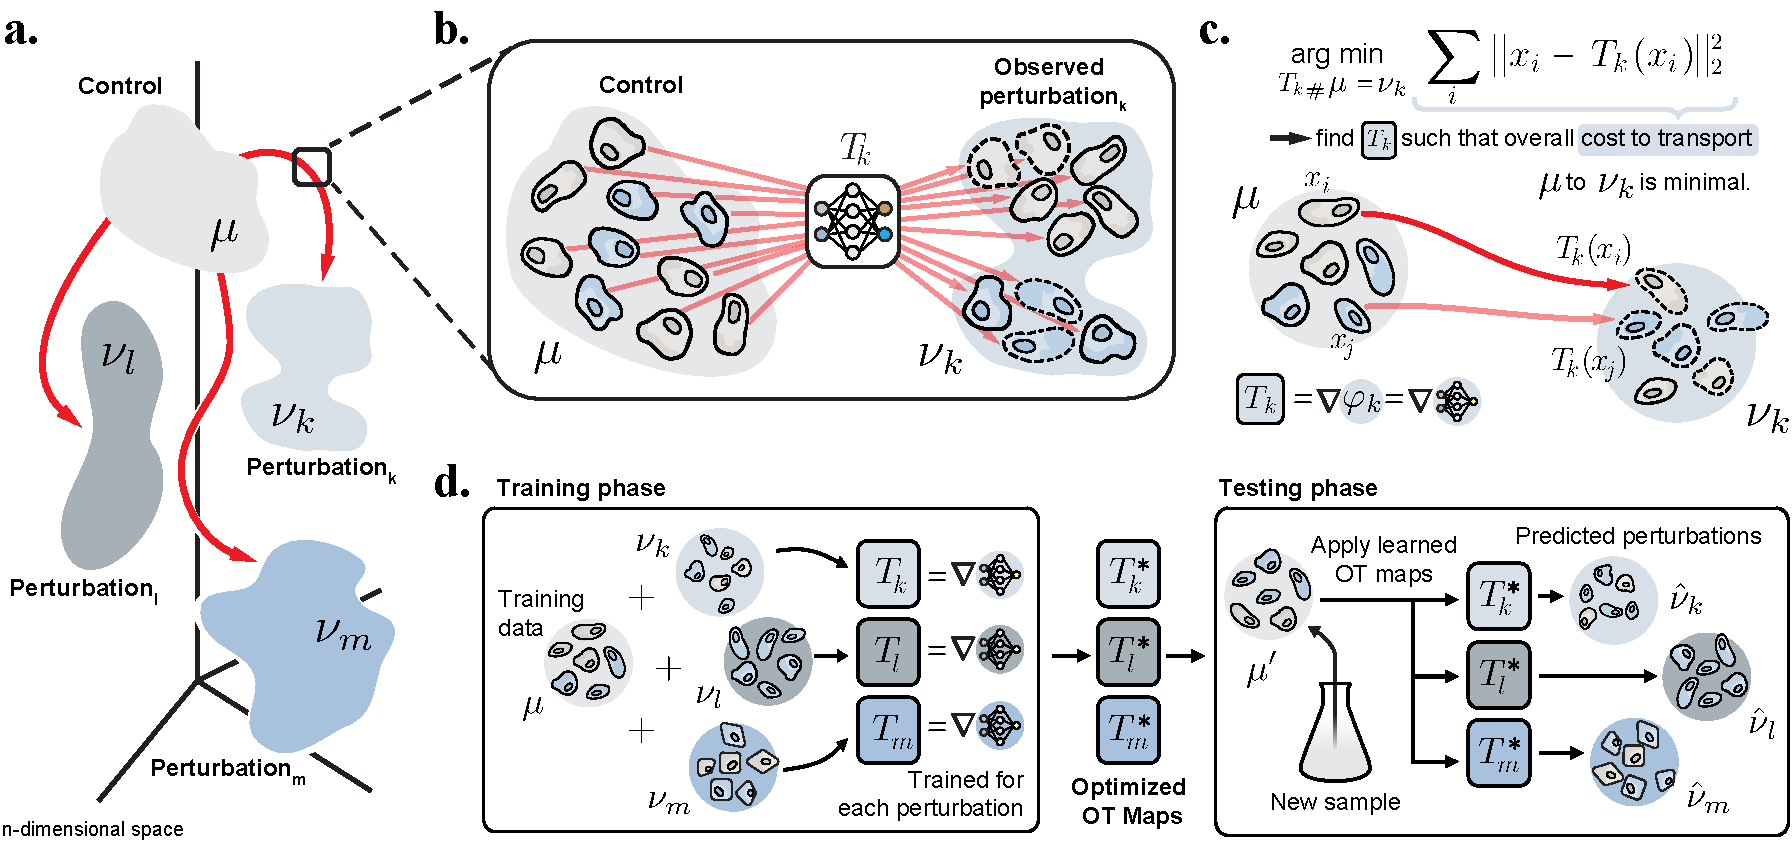
\includegraphics[width=\textwidth]{figures/fig_overview_cellot.pdf}
    \caption{\textbf{Overview of the \textsc{CellOT} Model.} \textbf{a.}~Distributions of single cells were measured in either an untreated control state ($\mu$) or in one of several perturbed states ($\nu_k, \nu_l, \nu_m,  \ldots$). These distributions lie in a high-dimensional space of profiled features. \textbf{b.}~For a perturbation $k$, we aim to model it with a function $T_k$ that maps untreated cells in $\mu$ to their treated counterparts in $\nu_k$. \textbf{c.}~Lacking paired measurements, we assume that the perturbation transforms $\mu$ into $\nu_k$ under a principle of minimal effort. In particular, we learn $T_k$ using optimal transport theory to directly estimate this distributional mapping as the gradient of the optimal transport dual potential $\nabla g_\theta$.
    \textbf{d.}~OT maps are learned for all perturbations independently. Because these maps are fully parameterized, \textsc{CellOT} can be trained, for example, on a set of initially provided samples to then make predictions on untreated cells originating from new, previously unseen samples.}
    \label{fig:overview_cellot}
\end{figure}


Characterizing and modeling perturbation responses at the single-cell level from non-time-resolved data remains one of biology's grand challenges. It finds applications in predicting cellular reactions to environmental stress or a patient's response to drug treatments. Accurate inference of perturbation responses at the single cell level allows us, for instance, to understand how and why individual tumor cells evade cancer therapies \citep{frangieh2021multimodal}. More generally, it deepens the mechanistic understanding of the molecular machinery that determines the respective responses to perturbations. Single-cell responses to genetic or chemical perturbations are  highly heterogeneous~\citep{liberali2014hierarchical} due to multiple factors, including pre-existing variability in the abundance and subcellular organization of mRNA and proteins~\citep{battich2013image, battich2015control, gut2018multiplexed, shaffer2017rare}, cellular states~\citep{kramer2019cellular}, and the cellular microenvironment~\citep{snijder2009population}. To effectively predict the drug response of each cell in a  population, whether derived from tissue culture or as primary cells from a patient biopsy, it is thus crucial to incorporate this heterogeneous multivariate subpopulation structure into the analysis.

\looseness -1 A fundamental difficulty in learning perturbation responses is that cells are usually fixed and stained or chemically destroyed to obtain these measurements. Hence, it is only possible to measure the same cells  before or after a perturbation is applied. 
Therefore, while we do not have access to a set of {\em paired} control/perturbed single-cell observations, we do have access to separate \emph{sets} of single-cell observations from control and perturbed cells, respectively. To subsequently match single cells between conditions and, at the same time, account for cellular heterogeneity is a highly complex pairing problem.

Here, we seek to learn a perturbation model that robustly describes the cellular dynamics upon intervention while still accounting for underlying variability across samples. Learning the responses on an existing patient cohort enables inference of treatment responses for new, i.e., previously unseen patients, assuming that we captured the heterogeneous drug reactions of patients during training.
It is crucial, however, to not simply model average perturbation responses of a patient cohort, but to capture the specificities of a single patient through personalized treatment effect predictions.
% Even though we seek a robust and coherent model, we must ensure that we propose personalized treatment effect predictions rather than average perturbation responses of a patient cohort possibly not capturing the specificities of a single patient.

\looseness -1 Previous methods to approximate single-cell perturbation responses fall short of solving this highly complex \emph{pairing} problem while, at the same time, accounting for cellular heterogeneity and the strong subpopulation structure of cell samples~\citep{wu2021single,gonzalez2020tumor,li2022single}. 
Current state-of-the-art methods~\citep{lopez2018scvi, lotfollahi2019scgen, yang2020predicting} predict perturbation responses via \emph{linear shifts} in a learned % low-dimensional
latent space.
While this can capture nonlinear cell-type-specific responses, the use of linear interpolations reduces the alignment problem to the possibly more challenging task of learning representations that are invariant to the corresponding perturbation. \\

\looseness -1 In this chapter, we introduce \textsc{CellOT}, a novel approach that predicts perturbation responses of single cells by \emph{directly} learning and uncovering maps between control and perturbed cell states, thus explicitly accounting for heterogeneous subpopulation structures in multiplexed molecular readouts.
Assuming perturbations incrementally alter molecular profiles of cells, such as gene expression or signaling activities, we learn these changes and alignments using a static \acrlong{OT} formulations (see \cref{sec:background_ot_static}). 
As described in \cref{sec:ot_for_biology}, it has found recent successes modeling cellular developmental processes~\citep{lavenant2021towards, schiebinger2019optimal}, albeit in a {\em non-parameterized} setting. Thus, such OT-based approaches are unable to make predictions on unseen cells, such as those from unseen samples, e.g., new patients. 
% One way to address the pairing problem is to assume that perturbed cellular states are coupled to their initial states under a principle of minimum action. That is, given unpaired observations of cells before and after perturbation, we would aim to pair cells to their treated states in such a way that the average distance between the pairs, in feature space, is minimal. This setting is ideally suited for acute cellular perturbations during which single cells do not redistribute entirely and randomly in multidimensional measurement space, but typically only in a few dimensions, maintaining the overall correlation structure.

\looseness -1 In the following, we propose a neural optimal transport-based approach for inferring single-cell perturbation responses. 
Our method, \textsc{CellOT}, learns an optimal transport map for each perturbation in a fully parameterized and highly scalable manner. Instead of directly learning a transport map~\citep{korotin2021wasserstein, yang2018scalable, prasad2020optimal}, \textsc{CellOT} parameterizes a pair of dual potentials \eqref{eq:dual-cvx} with convex neural networks \citep{amos2017input}. This choice induces an important theory-motivated inductive bias essential to model stability~\citep{makkuva2020optimal}. 

\looseness -1 We demonstrate \textsc{CellOT}'s effectiveness by (i.) learning single-cell marker responses to different cancer drugs in melanoma cell lines, (ii.) predicting single-cell transcriptome responses in biopsies of patients with systemic lupus erythematosus as well as Panobinostat treatment outcomes of glioblastoma patients, (iii.) inferring \acrfull{LPS} responses across different animal species, and (iv.) modeling the transcriptome evolution of cell fates in hematopoiesis. Moreover, we benchmark \textsc{CellOT} against current state-of-the-art methods on multiple tasks~\citep{lopez2018scvi, lotfollahi2019scgen, chen2020dissecting}.

\section{Neural Optimal Transport Solvers} \label{sec:neural_solvers}

To generalize optimal transport formulations to the out-of-sample setting, recent efforts have concentrated on developing parameterizations of neural optimal transport schemes.
While initial efforts concentrated on solving large-scale \acrshort{OT} problems \citep{seguy2018large}, the focus quickly moved to \acrfull{GAN} \citep{arjovsky2017wasserstein, genevay2018learning}.
The majority of existing methods thereby employ \acrshort{OT} as a loss function to compute the discrepancy between the model and the data (target) distribution. 
More recently, however, the focus has shifted to parameterizing the \acrshort{OT} map $T$ \eqref{eq:monge} \citep{yang2018scalable, rout2021generative, daniels2021score}. Such parameterized OT maps not only function as generative models but extend to tasks that involve interpolations between distributions. More concretely, neural network-based parameterizations of $T$ allow us to model the evolution from a measure $\mu$ into a measure $\nu$ \citep{tong2020trajectorynet}, i.e., the focus of this thesis.

Multiple strategies exist on how to parameterize the optimal transport problem.
In the following, we consider neural \acrshort{OT} solvers that make direct use of the \citeauthor{brenier1987decomposition} theorem (\cref{thm:brenier}) and are based on the semi-dual \eqref{eq:dual-cvx}. For a review of alternative approaches, see \cref{sec:other_neural_solvers}.
For convenience, let us restate the semi-dual formulation in \eqref{eq:dual-cvx}
\begin{equation*}
	\varphi^\star \leftarrow \arg\inf_{\varphi\, \text{convex}} \int \varphi \textrm{d}\mu + \int \varphi^*\textrm{d}\nu\,,
\end{equation*}
where the optimization problem is concerned with finding a convex function $\varphi$ and its convex conjugate \eqref{eq:legendre} $\varphi^*$ given by
\begin{equation} \label{eq:varphi_conjugate}
	\forall y, \quad \varphi^*(y) \defeq \sup _x \langle x, y\rangle-\varphi(y)\,.	
\end{equation}
As discussed in \cref{sec:background_brenier}, the optimal transport map $T^\star$ for cost $c(x,y) = \|x-y\|^2_2$ and $\gX = \gY = \mathbb{R}^d$ in~\eqref{eq:monge} can be recovered via $\nabla \varphi^\star$.

As the convex conjugate $\varphi^*$ is very hard to compute, \citet{makkuva2020optimal} propose to approximate it via another convex function $g$.
Thus, to learn the optimal transport map, the approach builds upon celebrated results by \citet{knott1984optimal} and \citet{brenier1991polar}, which relate the optimal solutions for the primal \eqref{eq:monge} and the dual form \eqref{eq:kantorovich-dual}, to derive a min-max formulation that approximates Monge map $T$ \citep[Theorem 3.3]{makkuva2020optimal}.
The resulting objective reads
\begin{equation} \label{eq:ot-minmax}
	\arg \max_{\varphi  \, \text{convex}} \min_{g \, \text{convex}}  -\int \varphi(x) \mathrm{d} \mu(x) -\int \langle y, \nabla g(y)\rangle - \varphi(\nabla g(y)) \,\mathrm{d} \nu(y)\,.
\end{equation}
The intuition behind the approach stems from the fact that
\begin{equation*}
	\int \varphi^*\textrm{d}\nu = \sup _{g \text{ convex}} \int \langle y, \nabla g(y)\rangle - \varphi(\nabla g(y))\,\mathrm{d} \nu(y)\,.
\end{equation*}
We observe that in $\langle y, \nabla g(y)\rangle - \varphi(\nabla g(y)) \leq \varphi^*(y)$ for all functions $g$ the equality is achieved with $g = \varphi^*$ \citep[Theorem 3.3]{makkuva2020optimal}. 

In order to solve the optimization problem stated in \eqref{eq:ot-minmax}, \citet{makkuva2020optimal} parameterize both potentials $\varphi$ and $g$ using \acrfull{ICNN} (\cref{sec:icnns}), i.e., neural networks that parameterize the class of convex functions \citep{amos2017input}, such that
\begin{align} \label{eq:cellot-optim}
	\nonumber \theta^\star, \phi^\star \leftarrow \arg \max_{\varphi_\theta  \, \text{convex}} \min_{g_\phi \, \text{convex}}  &-\int \varphi_\theta(x) \mathrm{d} \mu(x) -\int \langle y, \nabla g_\phi(y)\rangle \\
	&- \varphi_\theta(\nabla g_\phi(y)) \,\mathrm{d} \nu(y),
\end{align}
where $\theta$ and $\phi$ are the parameters of each \acrshort{ICNN}.
Thus, the potentials $\varphi$ and $g$ can be learned via an alternate min-max optimization problem with loss functions
% TODO: Double-check.
\begin{align} 
	\label{eq:makkuva_f_loss}
    \ell_\varphi(\mu, \nu; \theta) &= \mathbb{E}_{x \sim \mu}[\text{ICNN}_{\phi}(x)] - \mathbb{E}_{y \sim \nu}[\text{ICNN}_{\theta}(\nabla \text{ICNN}_{\phi}(y))],   \\
    \label{eq:makkuva_g_loss}
    \ell_g(\mu, \nu; \phi) &= -\mathbb{E}_{y \sim \nu}[\langle y, \nabla \text{ICNN}_{\phi}(y)\rangle-\text{ICNN}_{\theta}(\nabla \text{ICNN}_{\phi}(y))].
\end{align}
For more details, see \citet{makkuva2020optimal, korotin2021neural}.


\subsection{Convex Neural Architectures}
\label{sec:icnns}

Input convex neural networks are neural networks $\varphi_\theta(x)$ with specific constraints on the architecture and parameters $\theta$, such that their output is a convex function of some (or all) elements of the input $x$~\citep{amos2017input}. We consider  \acrshortpl{ICNN}, such that the output is a convex function of the entire input $x$. A typical \acrshort{ICNN} is a $L$-layer, fully connected network such that, for $l = 0, \dots, L-1$:
\begin{equation} \label{eq:icnn}
    z_{l+1} = a_l(W^x_lx + W^z_l z_l + b_l)  \text{ and } \varphi_\theta(x) = z_L,
\end{equation}
where by convention, $z_0$ and $W^z_0$ are $0$, $a_l$ are convex non-decreasing (non-linear) activation functions, $\theta=\{b_l, W^z_l, W^x_l\}_{l=0}^{L-1}$ are the weights and biases of the neural network, with weight matrices $W^z_l$ associated to latent representations $z$ that have non-negative entries. Since \citet{amos2017input}'s work, convex neural architectures have been further extended and shown to capture relevant models despite these constraints~\citep{amos2017input, makkuva2020optimal, huang2021convex}. In particular, \citet{chen2018optimal} provide a theoretical analysis that any convex function over a convex domain can be approximated in sup norm by an \acrshort{ICNN}.


\subsection{Alternative Approaches}
\label{sec:other_neural_solvers}

Learning optimal transport problems based on neural networks is at the core of many machine learning applications, including normalizing flows \citep{rezende2015variational,huang2021convex} and generative models \citep{arjovsky2017wasserstein, genevay2018learning}, albeit the transport map is not explicitly estimated.
% Here, the authors parameterize \textit{dual potentials} as Lipschitz neural networks, in the case $p=1$. In that case, the interplay between OT and estimation does not concern the map $T$ itself (which can be interpreted as a generator), but rather an auxiliary function (the discriminator). 
The formulation introduced in \cref{sec:neural_solvers} proposes a neural optimal transport scheme via the semi-dual formulation. In fact, a stream of foundational papers has proposed methods to approximate the dual potential with a neural network.
While a common strategies consists in parameterizing $\varphi$ through an \acrshort{ICNN} \citep{taghvaei20192, korotin2021wasserstein, makkuva2020optimal}, other works explore learning $\varphi$ using non-convex neural networks \citep{korotin2021neural, rout2021generative, nhan2019three}.
As the convex conjugate $\varphi^*$ is hard to compute, several strategies have been developed to solve the conjugation operation in \eqref{eq:varphi_conjugate}: \citet{taghvaei20192} thereby propose to exactly computing the conjugate, which, however, is computationally challenging. Besides approximations of the conjugate as considered in this thesis \citep{korotin2021wasserstein, makkuva2020optimal}, more recent approaches suggest (near-)exact conjugate computations through  amortized optimization \citep{amos2023amortizing}.

Beyond approaches that parameterize the dual potentials of optimal transport, several approaches consider parameterizing map $T$ directly. This is done either without any regularization \citep{yang2018scalable}, or by introducing regularizers that quantify how far a map $T_\theta$ deviates from the ideal properties we expect from a $c$-OT map.
More concretely, \citet{uscidda2023monge} introduce the Monge gap regularizer defined as
\begin{equation*}
	\int c(x, T_\theta(x)) \textrm{d} \mu(x) - W_c(\mu, T_\theta \sharp \mu)
\end{equation*}
that if 0 guarantees that $T_\theta$ is a $c$-OT map. For $c(x,y) = \|x-y\|^2_2$ and $\gX = \gY = \mathbb{R}^d$, for example, $T_\theta$ corresponds to a gradient of a convex function (\cref{thm:brenier}).


\section{Related Work}

\looseness -1 With increasing data availability, a diverse set of approaches has been proposed to model cellular perturbation responses, ranging from mechanistic to current deep learning-based approaches.
Mechanistic models \citep{yuan2021cellbox, frohlich2018efficient} define mathematical models of molecular interactions to model the effect of perturbation.
These methods, however, are restricted to simpler and well-understood systems as they do not capture highly nonlinear perturbation responses of a heterogeneous cell population. Further, these methods are limited in their applicability as they do not scale to genome-wide measurements \citep{snijder2012single, berchtold2018systems, green2016systems}.
Linear models \citep{dixit2016perturb, kamimoto2020celloracle}, on the other hand,  predict changes in cellular gene expression levels using regularized regression methods, where the model predicts a gene's expression level as a linear combination of effects of different perturbations, fitting the regulatory effect of each perturbation on each gene.
Due to assuming only linear relationships of individual genes in response to a perturbation, these methods are similarly  unable to capture complex and inhomogeneous population responses upon perturbation.
\citet{heydari2022iqcell}, on the other hand, predict perturbation responses by inferring the underlying gene regulatory network. Prediction of the perturbed states is achieved through a dynamic simulation of those logical gene networks. Thus, the predicted perturbed states are restricted to only the selected set of genes used to build the corresponding regulatory network.
Lastly, current state-of-the-art methods \citep{lopez2018scvi, lotfollahi2019scgen, yang2020predicting} aim to learn low-dimensional representations of inputs using autoencoders such that perturbation effects can be applied with simple linear interpolations in representation space. Thus, they predict perturbation responses via linear shifts in a learned low-dimensional latent space. These models are attractive because they are fully parameterized, enabling us to make predictions on unseen cells. By tackling the task of perturbation response predictions via the even more challenging task of learning a meaningful low-dimensional embedding, these methods can be expected to, at best, only perform moderately well. Therefore, we sought to learn a fully parameterized perturbation model that robustly describes the cellular dynamics upon intervention while accounting for underlying variability across samples.

\section{\textsc{CellOT}: Predicting Perturbation Responses via Neural Monge Maps}

In the following, we describe our approach, which uncovers single-cell perturbation responses by predicting couplings between control and perturbed cell states.
Hereby, let $\mathcal{X}$ denote the biological data space spanned by the measured cell features. We then treat a cell's response to perturbation $k$ as an evolution in a high-dimensional space of cell states $\mathcal{X} = \mathbb{R}^d$.

% we aim to learn the distribution of cells $\nu_k \in \mathcal{P}(\mathcal{X})$ upon some perturbation $k$, given a set of separate samples $\{ y_1^k, \dots, y_m^k \}, y_i^k \in \mathcal{X}$.
In formal terms, we denote the unperturbed control population by $\mu$ consisting of $n$ cells $x_i$ for $i = 1, \dots, n$, i.e., a dataset of $n$ observations $\{ x_1, \dots, x_n \}, x_i \in \mathcal{X}$ drawn from $\mu \in \mathcal{P}(\mathcal{X})$. Upon perturbation $k$, the multivariate state of each cell $x_i$ of the unperturbed population changes, which we observe as the perturbed population $\nu_k$ (\cref{fig:overview_cellot}a).
To understand the mode of action and effect of perturbations, we seek to learn the transition and alignment between populations $\mu$ and $\nu_k$ via parameterizing a map $T_k$ (see \cref{fig:overview_cellot}a-b), which explains the transition of each cell from the unperturbed cell population $\mu$ into their perturbed state $\nu_k$ upon treatment $k$.
Despite originating from  different observations, map $T_k$ determines for each cell $x_i$ the most likely corresponding cell $T_k(x_i)$ in the perturbed population (\cref{fig:overview_cellot}c).
Finding this map then not only allows us to model single-cell trajectories upon perturbation but also to predict the perturbed state of previously unseen control cells. As a result, we can forecast the outcome of a perturbation $k$  by applying the learned map $T_k$ to a new unperturbed population $\mu^\prime$ (\cref{fig:overview_cellot}d).

% Following \citet{makkuva2020optimal}, we learn the optimal map $T$ \eqref{eq:monge} between $\mu$ and $\nu_k$.
% Thus, instead of computing a coupling $\gamma$ individually for each pair of cell samples using existing solvers \citep{cuturi2013sinkhorn}, we learn a parameterized optimal transport map using neural networks. The parameterized OT map then serves as a robust predictor for cellular distribution shifts upon perturbations on unseen samples $\{x_i \}_{i=1}^{n^\prime} \sim \mu$, i.e., of another patient.

\looseness -1 The optimal map $T_k$ aligning the control and perturbed population, which we seek to find, should best describe the incremental changes in the multivariate profile of each cell after applying a perturbation $k$. Using optimal transportation theory \citep{villani2021topics, santambrogio2015optimal} to recover these maps and unveil single-cell reprogramming trajectories has been proposed as a strong modeling hypothesis in the domain of single-cell biology \citep{schiebinger2019optimal, cang2020inferring, demetci2022scot, huizing2022optimal, lavenant2021towards, zhang2021optimal}.
\begin{figure}
    \centering
    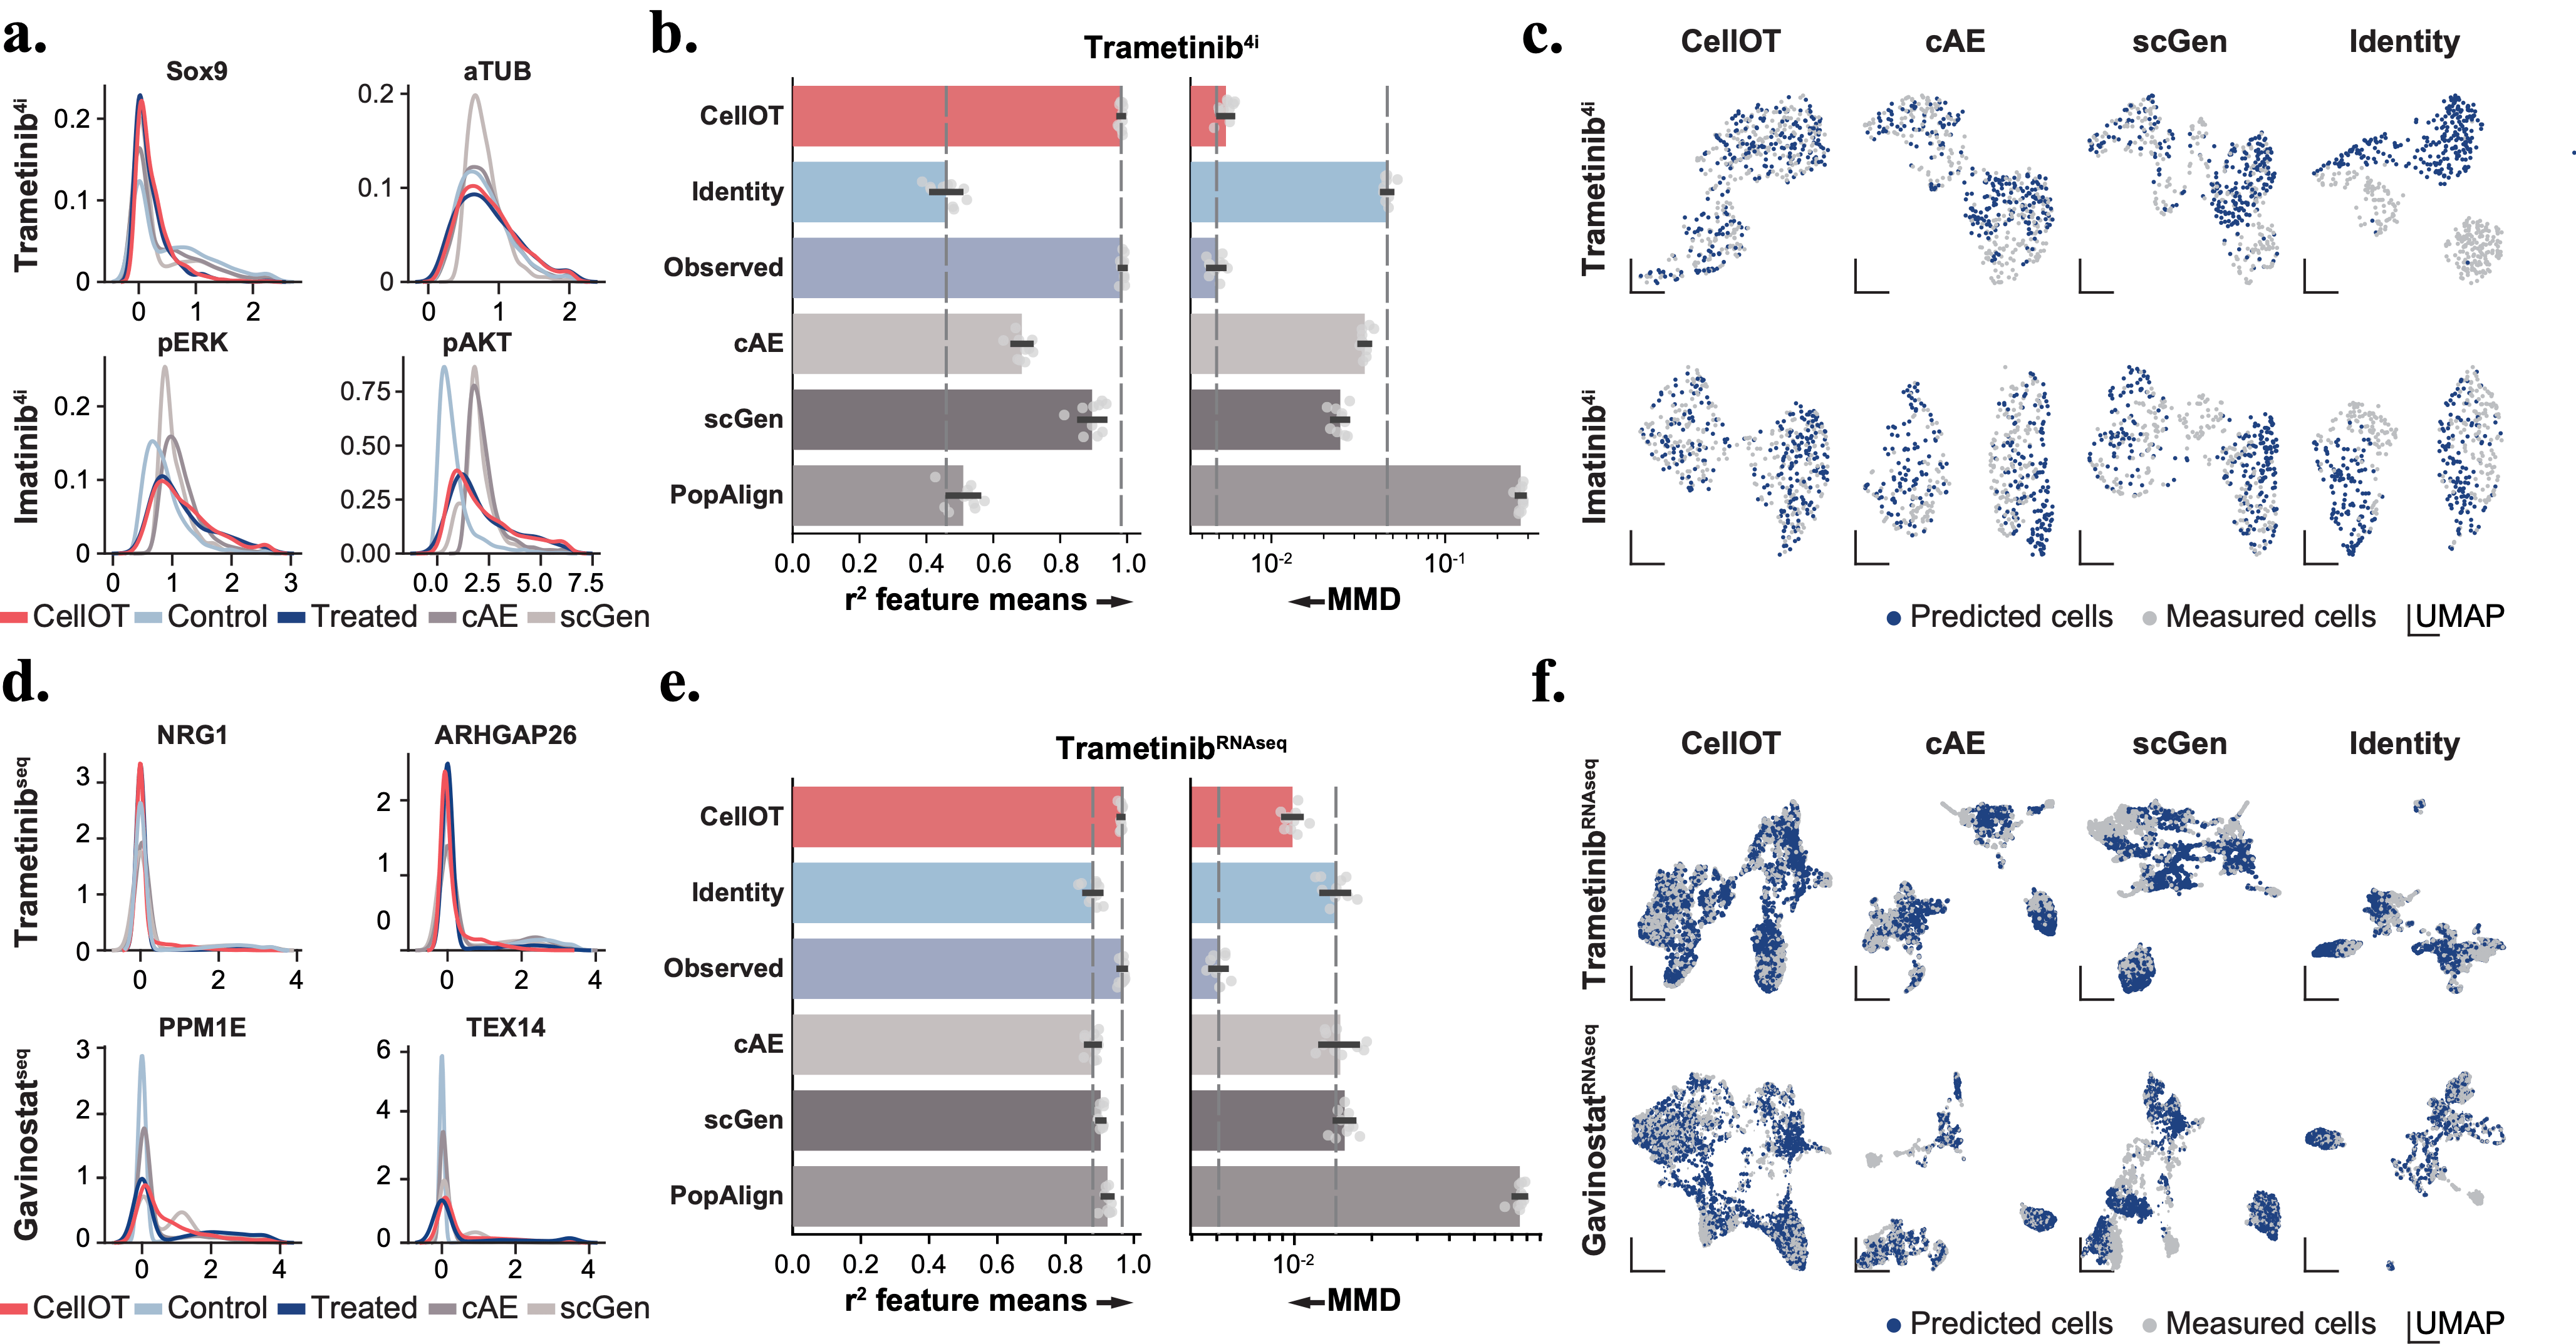
\includegraphics[width=\textwidth]{figures/fig_benchmark_cellot.png}
    \caption{\looseness -1 \textbf{\textsc{CellOT} outperforms current state-of-the-art methods on different data modalities.}  Marginal distribution of marker gene expression (x-axis) of cells profiled by \textbf{a.} 4i and \textbf{d.} scRNA. Observed control and treated states are shown in light and dark blue. \textsc{CellOT} predictions are shown in red and baseline predictions (scGen, cAE, PopAlign) are shown in gray. We compare models based on the distributional distance \acrshort{MMD} as well as average correlation coefficient $r^2$ between observed perturbed and predicted perturbed cells, for \textbf{b.} 4i and \textbf{e.} scRNA data. Error bars refer to the standard deviation over 10 bootstraps of the test set and the dashed lines correspond to the median of the identity and observed performances. Joint \acrshortpl{UMAP} of observed treated cells and cells predicted by each model for \textbf{c.} 4i and \textbf{f.} scRNA data. Projections are computed on a joint set of cells, down-sampled such that the number of observed perturbed (gray) and predicted perturbed cells (blue) are equal. An identity coupling compares treated cells to untreated cells. The analysis is conducted for the drugs Trametinib, Imatinib, and Gavinostat. 4i data was generated using cell lines M130219 and M130429.}
    \label{fig:benchmark_cellot}
\end{figure}
Optimal transport problems return the alignment between distributions $\mu$ and $\nu_k$ corresponding to the minimal overall cost between aligned molecular profiles, thus determining the most likely state of each cell upon perturbation (\cref{fig:overview_cellot}c).
$T_k$ is learned such that its image corresponds to $\nu_k$ and mass is moved from $\mu$ into $\nu_k$ according to a principle of minimal effort.
% Utilizing recent advancements in neural optimal transport theory, \textsc{CellOT} considers the dual form of the transport problem and parameterizes a pair of convex potentials with neural networks. $T_k$ is recovered as the gradient of one of these potentials.
As directly parameterizing the optimal transport map $T_k$ \citep{korotin2021wasserstein, yang2018scalable, prasad2020optimal} is unstable \citep[Table 1]{makkuva2020optimal}, we parameterize the convex potentials of the approximate semi-dual optimal transport problem $\varphi$ and $g$ \eqref{eq:ot-minmax}.
Given a set of perturbations $K$, and sample access to the control distribution $\mu$ as well as  distributions $\nu_k$ for each perturbation $k \in K$, \textsc{CellOT} learns the optimal pair of dual potentials $(\varphi_{\theta_k^\star}, g_{\phi_k^\star})$ by solving~\eqref{eq:cellot-optim}, each input convex neural networks \citep{amos2017input} is trained with loss functions \eqref{eq:makkuva_f_loss}-\eqref{eq:makkuva_f_loss}. We recover the optimal map $T_k$ using the gradient of a convex function $\varphi_k$, i.e., $\nabla \varphi_k$ \citep{makkuva2020optimal}.
% Using the learned convex potentials for each $k$, \textsc{CellOT} then predicts the transformation of a control cell $x_i$ upon perturbation $k$ via $\hat{y}_i^k = \nabla f_{\theta_k^\star}(x_i)$, i.e., samples following the predicted perturbed distribution $\hat{\nu_k} =(\nabla f_{\theta_k^\star})_{\sharp} \mu$. 

\section{Empirical Evaluation}

\subsection{Predicting Treatment Outcomes of Cancer Drugs}

\looseness -1 We apply \textsc{CellOT} to predict the responses of cell populations to cancer treatments using a proteomic dataset consisting of two melanoma cell lines (M130219 and M130429) \citep{raaijmakers2015new}, profiled by 4i~\citep{gut2018multiplexed}, and a scRNA-seq dataset~\citep{srivatsan2020massively}, which contain 34 and 9 different treatments, respectively.
% To put \textsc{CellOT}'s performance in perspective, we benchmark it against current state-of-the-art methods based on autoencoders \citep{lotfollahi2019scgen, lopez2018scvi}, which attempt to add perturbation effects through the manipulation of a learned latent representation.
We benchmarked \textsc{CellOT} against two autoencoder-based tools, \textsc{scGen}~\citep{lotfollahi2019scgen} and \textsc{cAE}~\citep{lopez2018scvi}, as well as \textsc{PopAlign}~\citep{chen2020dissecting}, a method based on aligning subpopulations of the control and treated space approximated through a mixture of Gaussian densities.
To further test the hypothesis of the optimal transport modeling prior, we compare the learned OT map $\nabla f_k$ for each perturbation $k$ with naive non-OT-based alignments.
Due to the high dimensional nature of scRNA-seq data, we apply $\textsc{CellOT}$ on latent representations learned by an autoencoder.
The marginal distributions for observed and predicted cell populations for two 4i treatments and two scRNA-seq treatments are shown in \cref{fig:benchmark_cellot}a, d. 
Two features are selected for each perturbation.
While the autoencoder baselines tend to capture the mean of the treated cell population, they are less successful in matching all heterogeneous states of the perturbed population, i.e., higher moments of the perturbed population.
% More precisely, these methods do not capture higher moments of the perturbed population, as for example the standard deviation of phosphorylated AKT (pAKT) levels of Imatinib-treated 4i cells. 
Thus, these models tend to learn over-simplified perturbation effects and are insufficient when aiming to understand heterogeneous rather than average cellular behaviors.
\textsc{CellOT}, on the other hand, is able to capture these higher moments, yielding accurate and nuanced predictions.

 \begin{figure}
     \centering
     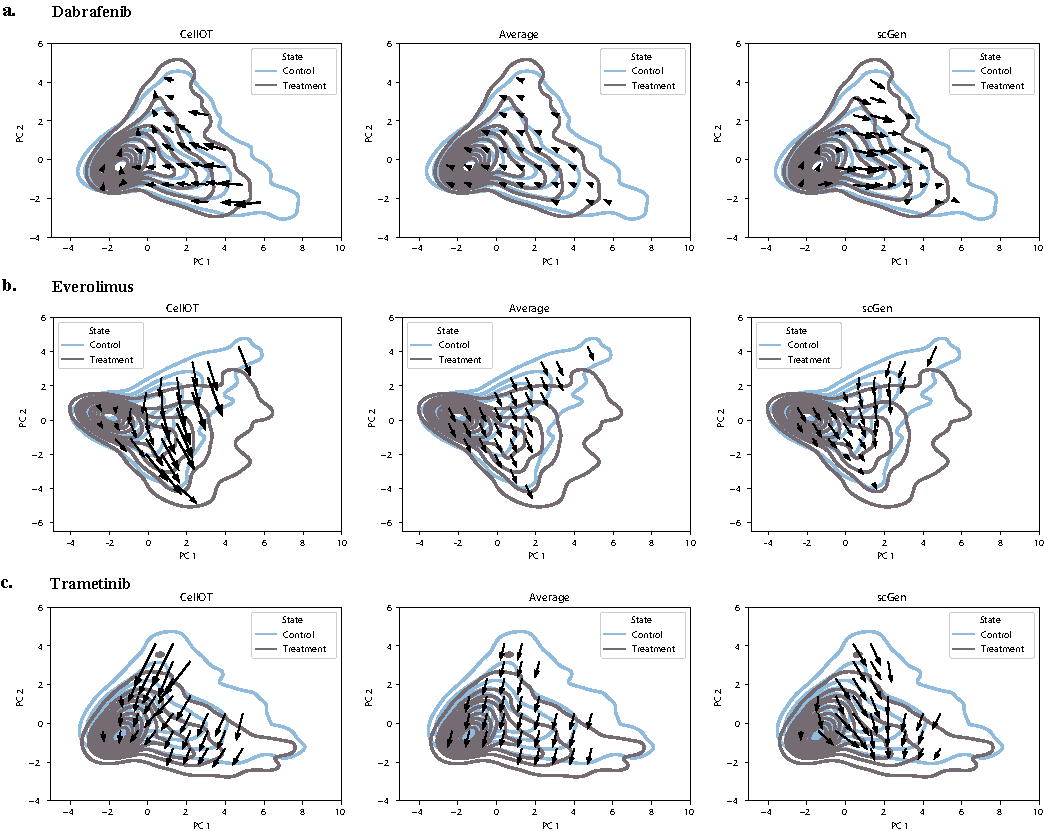
\includegraphics[width=\textwidth]{figures/fig_4i_vector_fields.pdf}
     \caption{Visualization of the learned vector field describing the perturbation response on the single-cell level for \textbf{a.} Dabrafenib, \textbf{b.} Everolimus, and \textbf{c.} Trametinib of the 4i dataset for \textsc{CellOT}, the average effect, and \textsc{scGen} on the first two principal components. Cellular responses are computed as the predicted treated state minus the observed control state for each individual cell. Arrow tails are placed in a grid within PC space and arrow heads correspond to the average response of cells within each neighborhood, projected into PC space.}
     \label{fig:4i_vector_fields}
 \end{figure}

\looseness -1 This can be further quantified % differences between the distributions of observed and predicted treated cell populations, we determine 
through distributional metrics such as the \acrfull{MMD} \citep{gretton2012kernel}.
Low values of \acrshort{MMD} imply that all moments of two distributions are matched, and thus the entire distribution of perturbed cells is captured in fine detail, beyond the population average.
The \acrshort{MMD}s between the predicted and observed populations for the selected perturbations are shown in \cref{fig:benchmark_cellot}b, e.
For scRNA-seq data, \acrshort{MMD} evaluations are computed using the top 50 marker genes.
In addition to the autoencoder baselines, we include the trivial \emph{identity} baseline that predicts treatment effects simply by returning the untreated states,
as well as a theoretical lower bound, \emph{observed}, comprising a different set of observed perturbed cells, thus only varying from the true predictions up to experimental noise.
We find that \textsc{CellOT} can approach the lower bound (\emph{observed} setting), while the baseline methods often do not improve much over the \emph{identity} setting.
Fig. \ref{fig:4i_vector_fields} visualizes the learned maps, % projected onto the first two principal components, 
further demonstrating \textsc{CellOT}'s ability to model fine-grained responses.


\looseness -1 Finally, we compute \acrfull{UMAP} projections~\citep{umap} on a joint set of predicted and observed perturbed cells utilizing the full feature space, shown in \cref{fig:benchmark_cellot}c, f.
We observe that the perturbed cell states inferred by \textsc{CellOT} are well integrated with the observed perturbed cells. Again, both baselines do not recover the perturbed distribution in its entirety % (via higher order moments)
and thus the perturbed state of different subpopulations is not captured consistently.
$\textsc{CellOT}$ outperforms the baselines in both metrics across all treatments, typically by one order of magnitude.
We attribute the strong performance of \textsc{CellOT} to its ability to learn a transport function that considers explicitly the data geometries of cell populations through the theory of optimal transport.

\subsection{Capturing Cell-to-Cell Variability in Drug Responses}
\looseness -1 Capturing distinct perturbation responses of different cell types within the same sample remains a challenging computational task. To reduce the task's complexity, prediction algorithms can be guided by predefined cell type labels both in the perturbed and unperturbed states \citep{chen2020dissecting} or set to approximate the mean drug response \citep{lotfollahi2019scgen}.  These simplifications come at a cost: the reliance on a priori knowledge about present and relevant cell types, the assumption that cell types are characterized by the same features before and after a perturbation, and that the drug response is uniform within a cell type.
In the worst case, these limitations risk masking true and important drug response heterogeneity  and thus hamper the discovery of novel cell types or cell state-specific perturbation responses.

\textsc{CellOT} is free of these limitations and enables scientists to query the predicted single-cell responses at the granularity best suited to answer their biological questions. As a proof of concept, we co-cultured the aforementioned patient-derived melanoma cell lines at equal ratios and performed a boutique drug screen, during which we exposed cells 8h to a panel of 34 drugs and measured the single-cell drug responses with the 4i technology. 
Using \textsc{CellOT}, 
% and cells from both cell lines, 
we predict the perturbed cell states of a shared set of control (DMSO-treated) cells (\cref{fig:biological_analysis}a) for each drug.
Previous work \citep{kramer2019cellular} shows that phosphorylation levels of signaling kinases upon drug treatments are tightly linked to the cellular state. 
To assess whether this relationship was retained in predicted compared to observed perturbed cells, we analyzed the phosphorylation levels of extracellular signal-regulated kinases (pERK) using the transport maps learned by \textsc{CellOT} on each drug.
Using 750 predicted and 750 observed perturbed cells, we computed \acrshort{UMAP} projections joint-wise from all features except pERK. \cref{fig:biological_analysis}b shows the predicted and observed population individually annotated with the respective pERK levels of each cell. We find the spatial organization of the two projections to look almost identical and that pERK levels had a highly comparable distribution across the cells of either class and all drug treatments (further analysis in \cref{fig:4i_analysis_extended}a, b).
% We furthermore supplemented this analysis by faithfully reconstructing unseen pERK levels of predicted cells from their local neighborhoods in multidimensional feature space

% Based on the 3 nearest neighbors computed using all features except pERK, we show that these features of importance are faithfully reconstructed by observed cells in the local neighborhood of each predicted cell, thus, retaining the crucial connection between kinase activity levels and cellular states.

% \subsection*{\textsc{CellOT} enables cell state-aware drug profiling and disentangles subpopulation-specific drug effects}
\subsection{Disentangles Subpopulation-Specific Drug Effects}
\textsc{CellOT} allows us to 
% profile the severity of drug perturbations on individual cellular states and understand how the cellular state of unperturbed cells determines drug response behavior. We can 
isolate the mode of action of each drug by computing the difference between predicted perturbed cells and untreated control cells. % , i.e., the \emph{cost} of the optimal transport.
A \acrshort{UMAP} embedding of all cells color-coded by the treatment distinctly separates different treatments (Figs.~\ref{fig:biological_analysis}c and \ref{fig:4i_analysis_extended}e), all of which \textsc{CellOT} is able to faithfully learn.
Such distinct treatment embeddings are not present when accounting only for an average perturbation effect (\cref{fig:4i_analysis_extended}d), indicating the importance of capturing the cellular heterogeneity of drug responses.

\looseness -1 Using Leiden clustering on the full feature set, we grouped unperturbed control cells in 12 cellular states (\cref{fig:biological_analysis}d, \cref{fig:4i_analysis_extended}g). Cellular states 1, 5, 6, 9, and 12 show high levels of MelA and no SOX9 and thus correspond to the melanocytic cell line M130429, whereas the SOX9\textsuperscript{+} and MelA\textsuperscript{-} states 2, 3, 4, 7, 8, 10, and 11 represent the mesenchymal cell line M130219. Overall, we find that M130429 cells have higher phosphorylation levels of the measured signaling kinases compared to M130219;
% The cluster structure derived from the control cells is further persistent in the perturbed states. 
a stereotypical spatial organization of cellular states is retained for the majority of the drugs,  and cell states belonging to the same cell line cluster together (\cref{fig:4i_analysis_extended}f). 

\begin{figure}
    \centering
    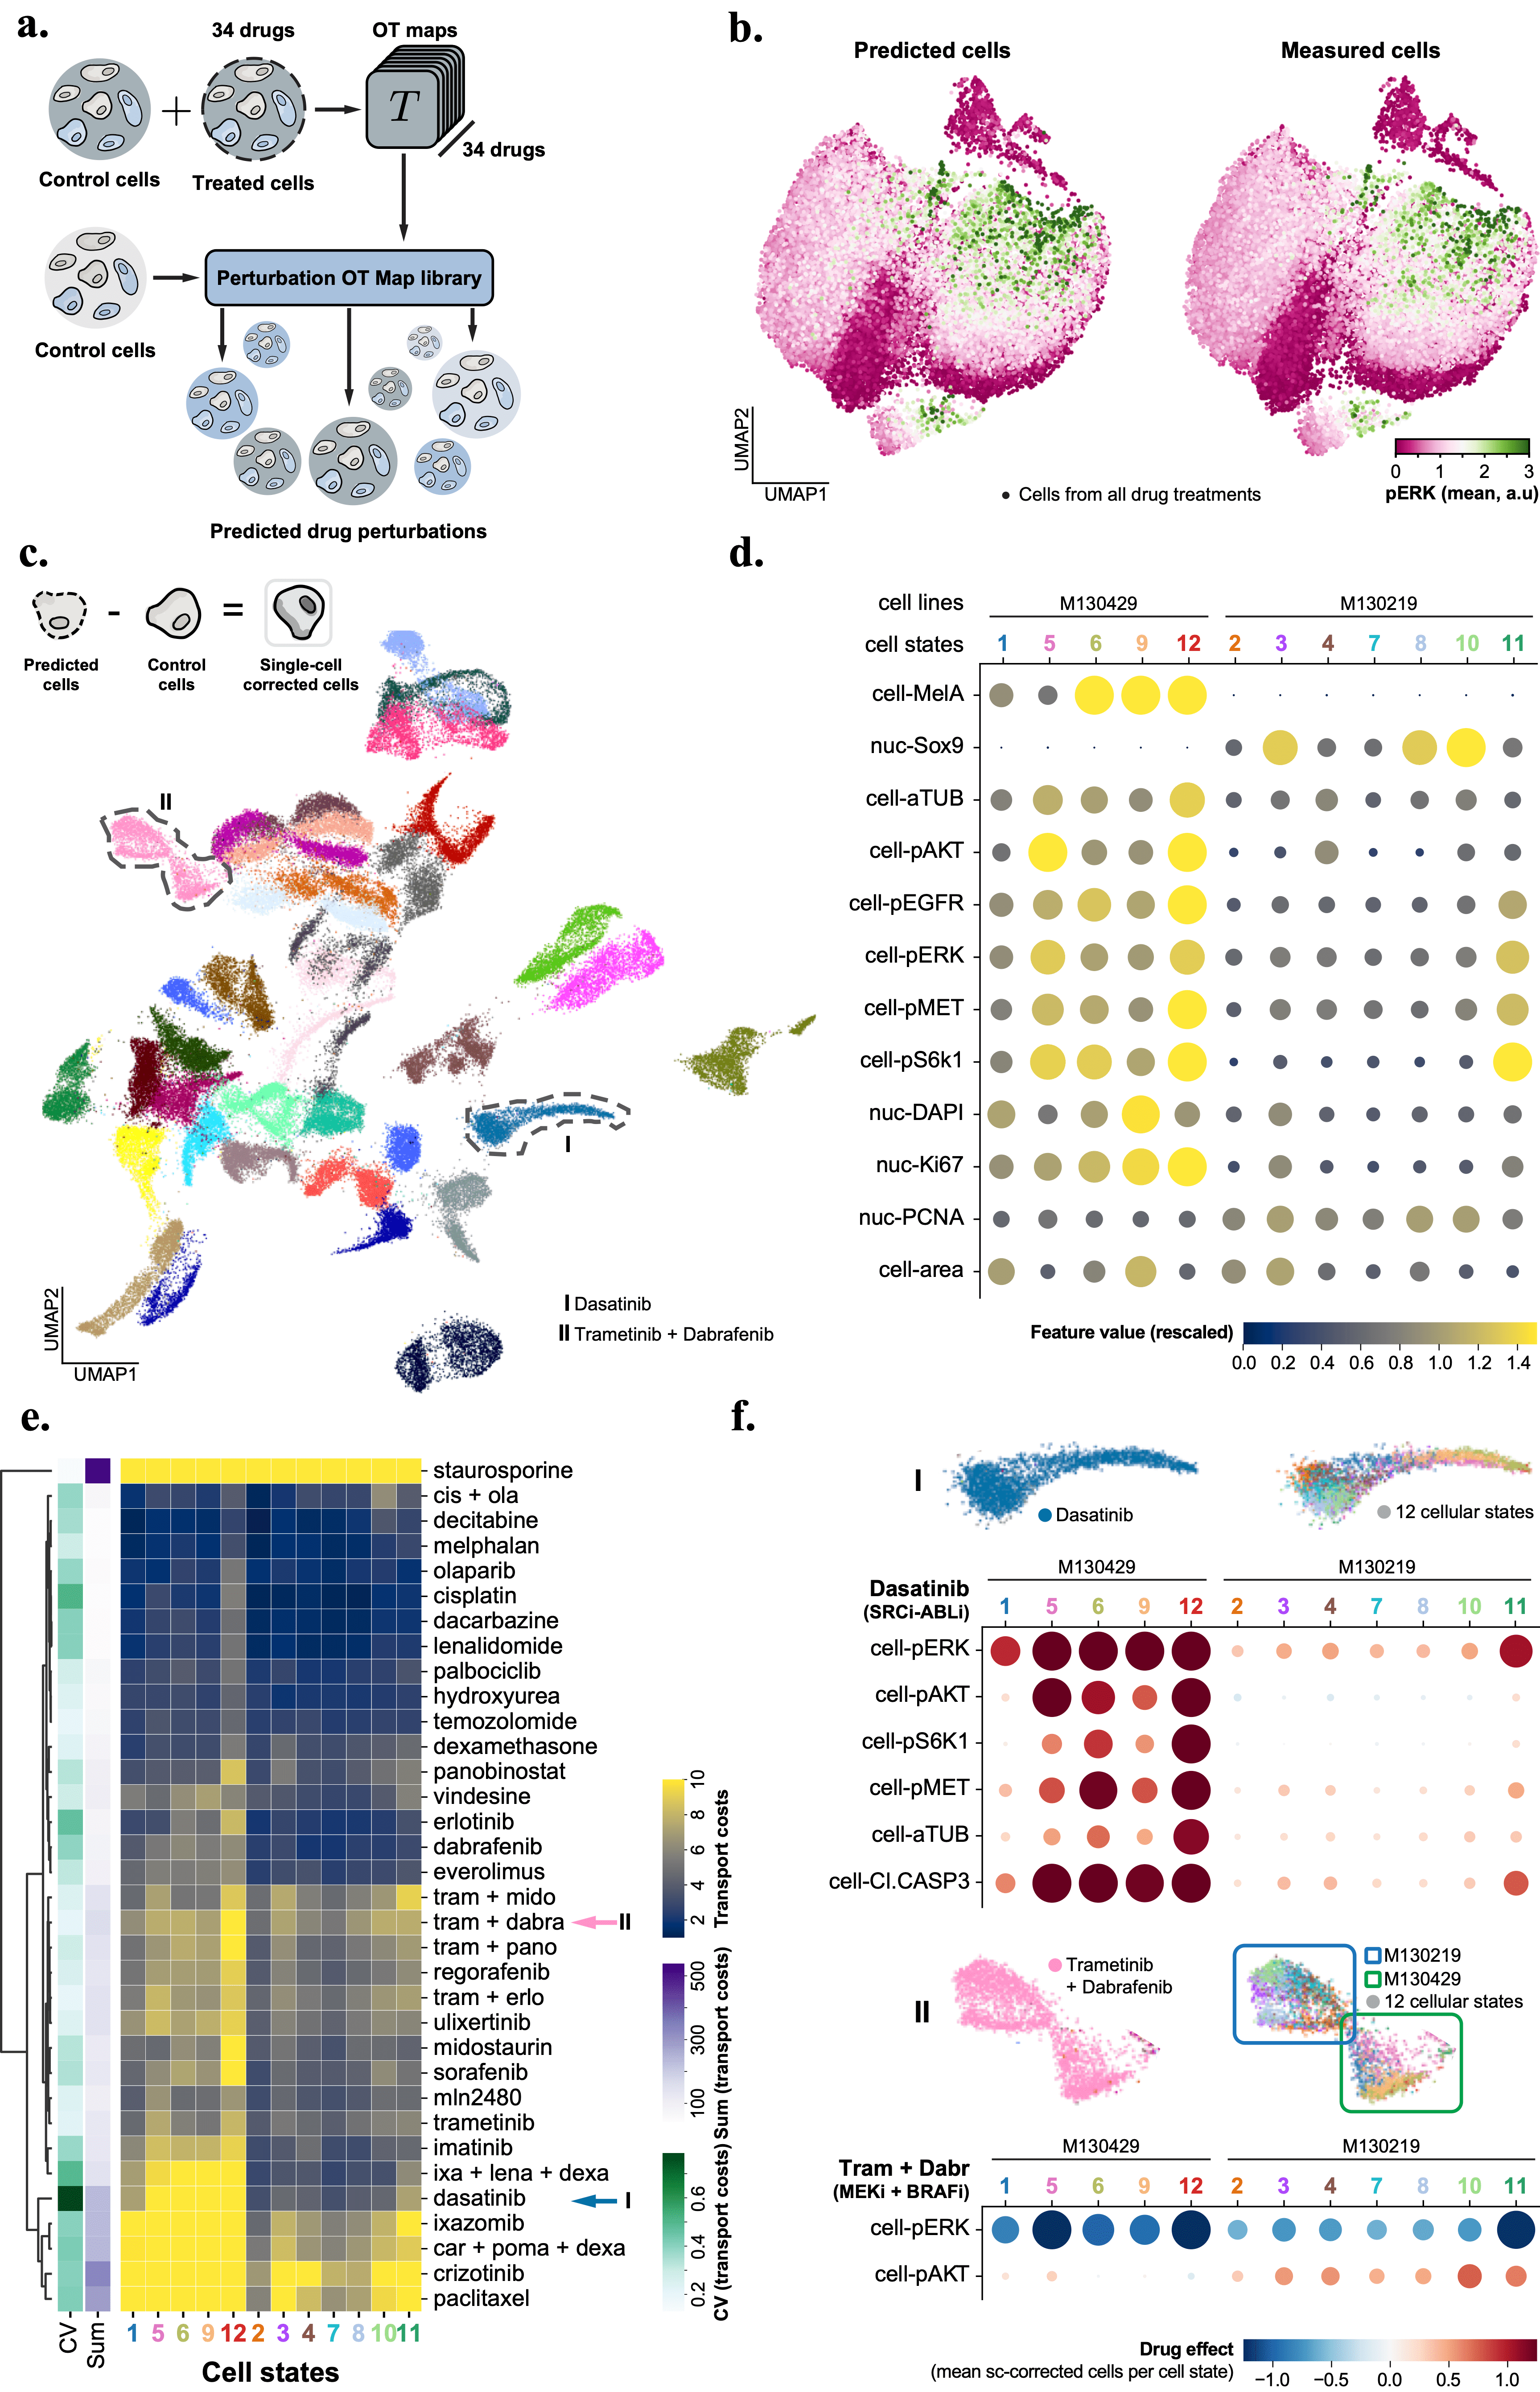
\includegraphics[width=\textwidth]{figures/fig_biological_analysis.png}
\end{figure}
\captionof{figure}{
\looseness -1 \textbf{CellOT facilitates the multiplexed single-cell characterization of cancer drugs.} 
    \textbf{a.} \textsc{CellOT} training and prediction setup. 34 \textsc{CellOT} models were trained, one for each drug perturbation. Subsequently, each model was used to predict perturbed cells from a common set of unseen control cells. \textbf{b.} \acrshort{UMAP} projection constructed with equal numbers of predicted and measured cells from 34 perturbations. Dots correspond to cells, color-coded for measured or predicted pERK intensity, \textbf{c.} \acrshort{UMAP} projection of single-cell perturbation effects using predicted cells. Dots correspond to cells, color-coded for drug treatment (see \cref{fig:4i_analysis_extended} for a full legend for single-cell perturbation effect calculation). \textbf{d.} Cell states identified in control cells. Each column represents a cell state. Horizontal axis, cell states are sorted based on their association with the cell lines M130219 and M130429.  Vertical axis, cellular features (see \cref{fig:4i_analysis_extended} for the full feature set). The size and hue of the circles are scaled on the feature values. \textbf{e.} Clustergram of transport cost (TC) of drug treatments for each cell state (main heatmap, blue-yellow color scheme), the sum of TCs (Sum) of all states per drug (first column left of the heatmap, purple), the coefficient of variation (CV) of TCs per drug (second column left of the heatmap, green) and the dendrogram based on the hierarchical clustering the drug's cell state TCs. Cell states are sorted as in \textbf{d}. \textbf{f.} Cell state-specific responses to drug treatments. Top panel (I) Dasatinib. Bottom panel (II) Trametinib + Dabrafenib. Panel organization: top-left, condition-focused enlargement of \acrshort{UMAP} projection from \textbf{c}. Top-right, same as top-left but color-coded for cell state assignment. Bottom, columns represent a cell state,  rows highlighted features. `cell-' stands for mean cell intensity. Circles are scaled based on drug effect size, the stronger the effect the larger the circles. Negative values are encoded in hues of blue, and positive values in red hues of the respective circles. \vspace{10pt}}
\label{fig:biological_analysis}
\looseness -1 Computing the difference between the control and treated state of each drug, i.e., the optimal
% what corresponds to the 
transport cost, allows us to further characterize a drug's severity. 
% High overall transport costs correspond to large feature value changes, i.e., a strong perturbation effect. 
Apoptosis inducers (e.g., Staurosporine), proteasome inhibitors (e.g., Ixazomig and Carfilzomib or the combination treatment Carfilzomib + Pomalidomide + Dexamethasone), microtubule-stabilizing agents (e.g., Paclitaxel), c-Met inhibitors (e.g., Crizotinib), and ATP competitors for multiple tyrosine kinases such as c-KIT, and Bcr-Abl (i.e., Dasatinib) show high transport costs and thus substantial feature changes in all cellular states (\cref{fig:biological_analysis}e). Other drugs demonstrate less severe effects in the observed 8h incubation period. 
% Nonetheless, we find that most  drugs affect multiple cellular states and that individual cellular states have varying sensitivities to drugs in the drug panel.
We find all perturbations to increase levels of cleaved Caspase 3, an apoptosis marker, in various cellular states and in both cell lines (\cref{fig:4i_analysis_extended}k), with the exception of Dasatinib, which specifically induced cell death in cellular states 5, 6, 9, and 19 associated to M130429 (\cref{fig:biological_analysis}f).


\looseness -1 Previous work by \citet{smith2016inhibiting} reports that M130429 cells reduce metabolic activity % (a proxy of cell viability)
upon treatment with inhibitors of MEK (MEKi) and RAF (RAFi), while M130219 cells are resistant to these inhibitors. When comparing the responses of the two cell lines to Trametinib (MEKi) and MLN2480 (panRAFi) in the MEK and PI3K pathway using pERK and pAKT as the respective readouts, we find that MEKi-sensitive M130429 cells down-regulate pAKT and pERK, whereas the MEKi-resistant M130219 cells only down-regulate pERK. Consistently, we also find that treatment with MLN2480 results in a similar differential drug response (\cref{fig:4i_analysis_extended}i). This suggests that \textit{decoupling} of the MEK and PI3K pathways may confer resistance to MEK and Raf inhibitors and constitute an adaptation to the escape of cancer therapy \citep{kun2021mek}. We find further supporting evidence of pathway crosstalk alteration when we analyze pAKT and pERK levels upon treatment with a cocktail of Trametinib (MEKi) and Dabrafenib (BRAFi). 

\looseness -1 In response to two drugs impinging on the MEK pathway, we observe pERK to be reduced in both cell lines but increased pAKT levels in the MEKi-resistant cell line M130219 (which resistance was acquired during pre-exposing a patient to MEKi) (\cref{fig:biological_analysis}f). This finding points towards a compensatory feedback mechanism acquired by M130219 during MEKi treatment by which inhibition of the MEK pathway (quantified as a reduction of pERK) would stimulate signaling through the PI3K pathway, possibly through activation of an upstream receptor kinase \citep{caunt2015mek1}. 
Our results on two co-cultured primary melanoma cell lines treated with various anti-cancer drugs show that \textsc{CellOT} can accurately capture phenotypic heterogeneity in unperturbed cell populations and predict diverse drug responses by incorporating the underlying cell-to-cell variability without predefined cell line labels. 
% Further, we find that \textsc{CellOT} reveals differential drug responses between the cellular states of the same cell lines, thus showcasing its ability to reveal unknown cell state-associated drug responses in an unsupervised fashion.
    
% \subsection*{\textsc{CellOT} accurately predicts single-cell responses for unseen patients}
\subsection{Inferring Cellular Responses in Unseen Patients}
The maps between molecular states before and after treatments learned by \textsc{CellOT} contribute to a better understanding of the differences between cells that respond to certain drugs and cells that do not respond. This is crucial for inferring an incoming patient's response to drugs and settings with high cell-to-cell variability.
To make predictions on unseen patients, however, we need to demonstrate that the learned maps $T$ model perturbation responses across different patients coherently and robustly, while still predicting personalized treatment outcomes for each patient instead of mere population averages.

% TODO: Check acronyms.
To test the generalization capacity of \textsc{CellOT} in such an \acrfull{oos} scenario, we use a \acrfull{PBMC} droplet scRNA-seq dataset. \citet{kang2018multiplexed} characterize the cell type specificity and inter-individual variability of the response of eight lupus patients to interferon beta (IFN-$\beta$), a potent cytokine that induces genome-scale changes in immune cell transcriptional profiles. 
% The dataset contains two pools, IFN-$\beta$-treated and control, prepared with the same number of cells from each individual, thus allowing us to investigate the cell fate differences between unperturbed and perturbed cells.
In the following, we compare the performance of \textsc{CellOT} and other baselines in an \acrfull{iid} setting, where models see cells from all patients, as well as in the out-of-sample setting, where models do not see cells from a specific holdout patient (see \cref{fig:generalization_cellot}a).
% A robust method should show little to no performance drop from the i.i.d. to the o.o.s. scenario.
    
As in the previous analysis, we evaluate how accurately \textsc{CellOT} captures the change in the overall expression of different marker genes from control to IFN-$\beta$-treated cells and thus how well the predicted gene expression marginals are aligned with the treated population (\cref{fig:generalization_cellot}b). Here, we consider the genes \textit{CXCL11}, \textit{CCL2}, and \textit{APOBEC3A},
since they are connected with autoimmune diseases, including systemic lupus erythematosus \citep{hedrich2011epigenetic, perez2021sustained}
and thus potential therapeutic targets
in the management of patients with lupus and, likely, other interferonopathies \citep{mathian2015targeting,rani1996characterization,hedrich2011epigenetic,mathian2015targeting,perez2021sustained,flier2001differential}.
% CXCL11 and CCL2 are both chemokines
These selected genes show a large change in expression from the control to the perturbed population, partially exhibiting a bimodal gene expression profile upon perturbation. In contrast to \textsc{CellOT}, the baselines do not accurately predict these large transcriptomic shifts of these genes.


\looseness -1 All models, including \textsc{CellOT}, show little performance drop when modeling the treatment outcome on a new patient using the generalized perturbation model $T_L$ trained on the patient cohort and using the control cells $\mu_z$ of the unseen patient as input.
This becomes evident when comparing the predicted population $\hat{\nu}_z$ with observations $\nu_z$ using the \acrshort{MMD} metric. \cref{fig:generalization_cellot}c displays summary results in which each individual patient was considered for the holdout set. \textsc{CellOT} outperforms previous baselines both in the i.i.d.~and in the o.o.s.~setting, while further showing a smaller performance drop when generalizing to the unseen patient.
These results suggest that the learned optimal transport maps correctly model the shift in the structures of the cellular subpopulation present in all patients, thus robustly performing out-of-sample.
We repeat the same evaluation for a glioblastoma cohort consisting of seven patients \citep{zhao2021deconvolution}. However, generalization within this setting proved to be difficult for \textsc{CellOT} and all baselines, due to the small size of the cohort and high degree of variance within the responses of each individual. 
% We have identified under which conditions generalization to unseen patients is feasible. 
For a complete analysis, see \cref{fig:gbm_patients_iid_ood}.

\begin{figure}
    \centering
    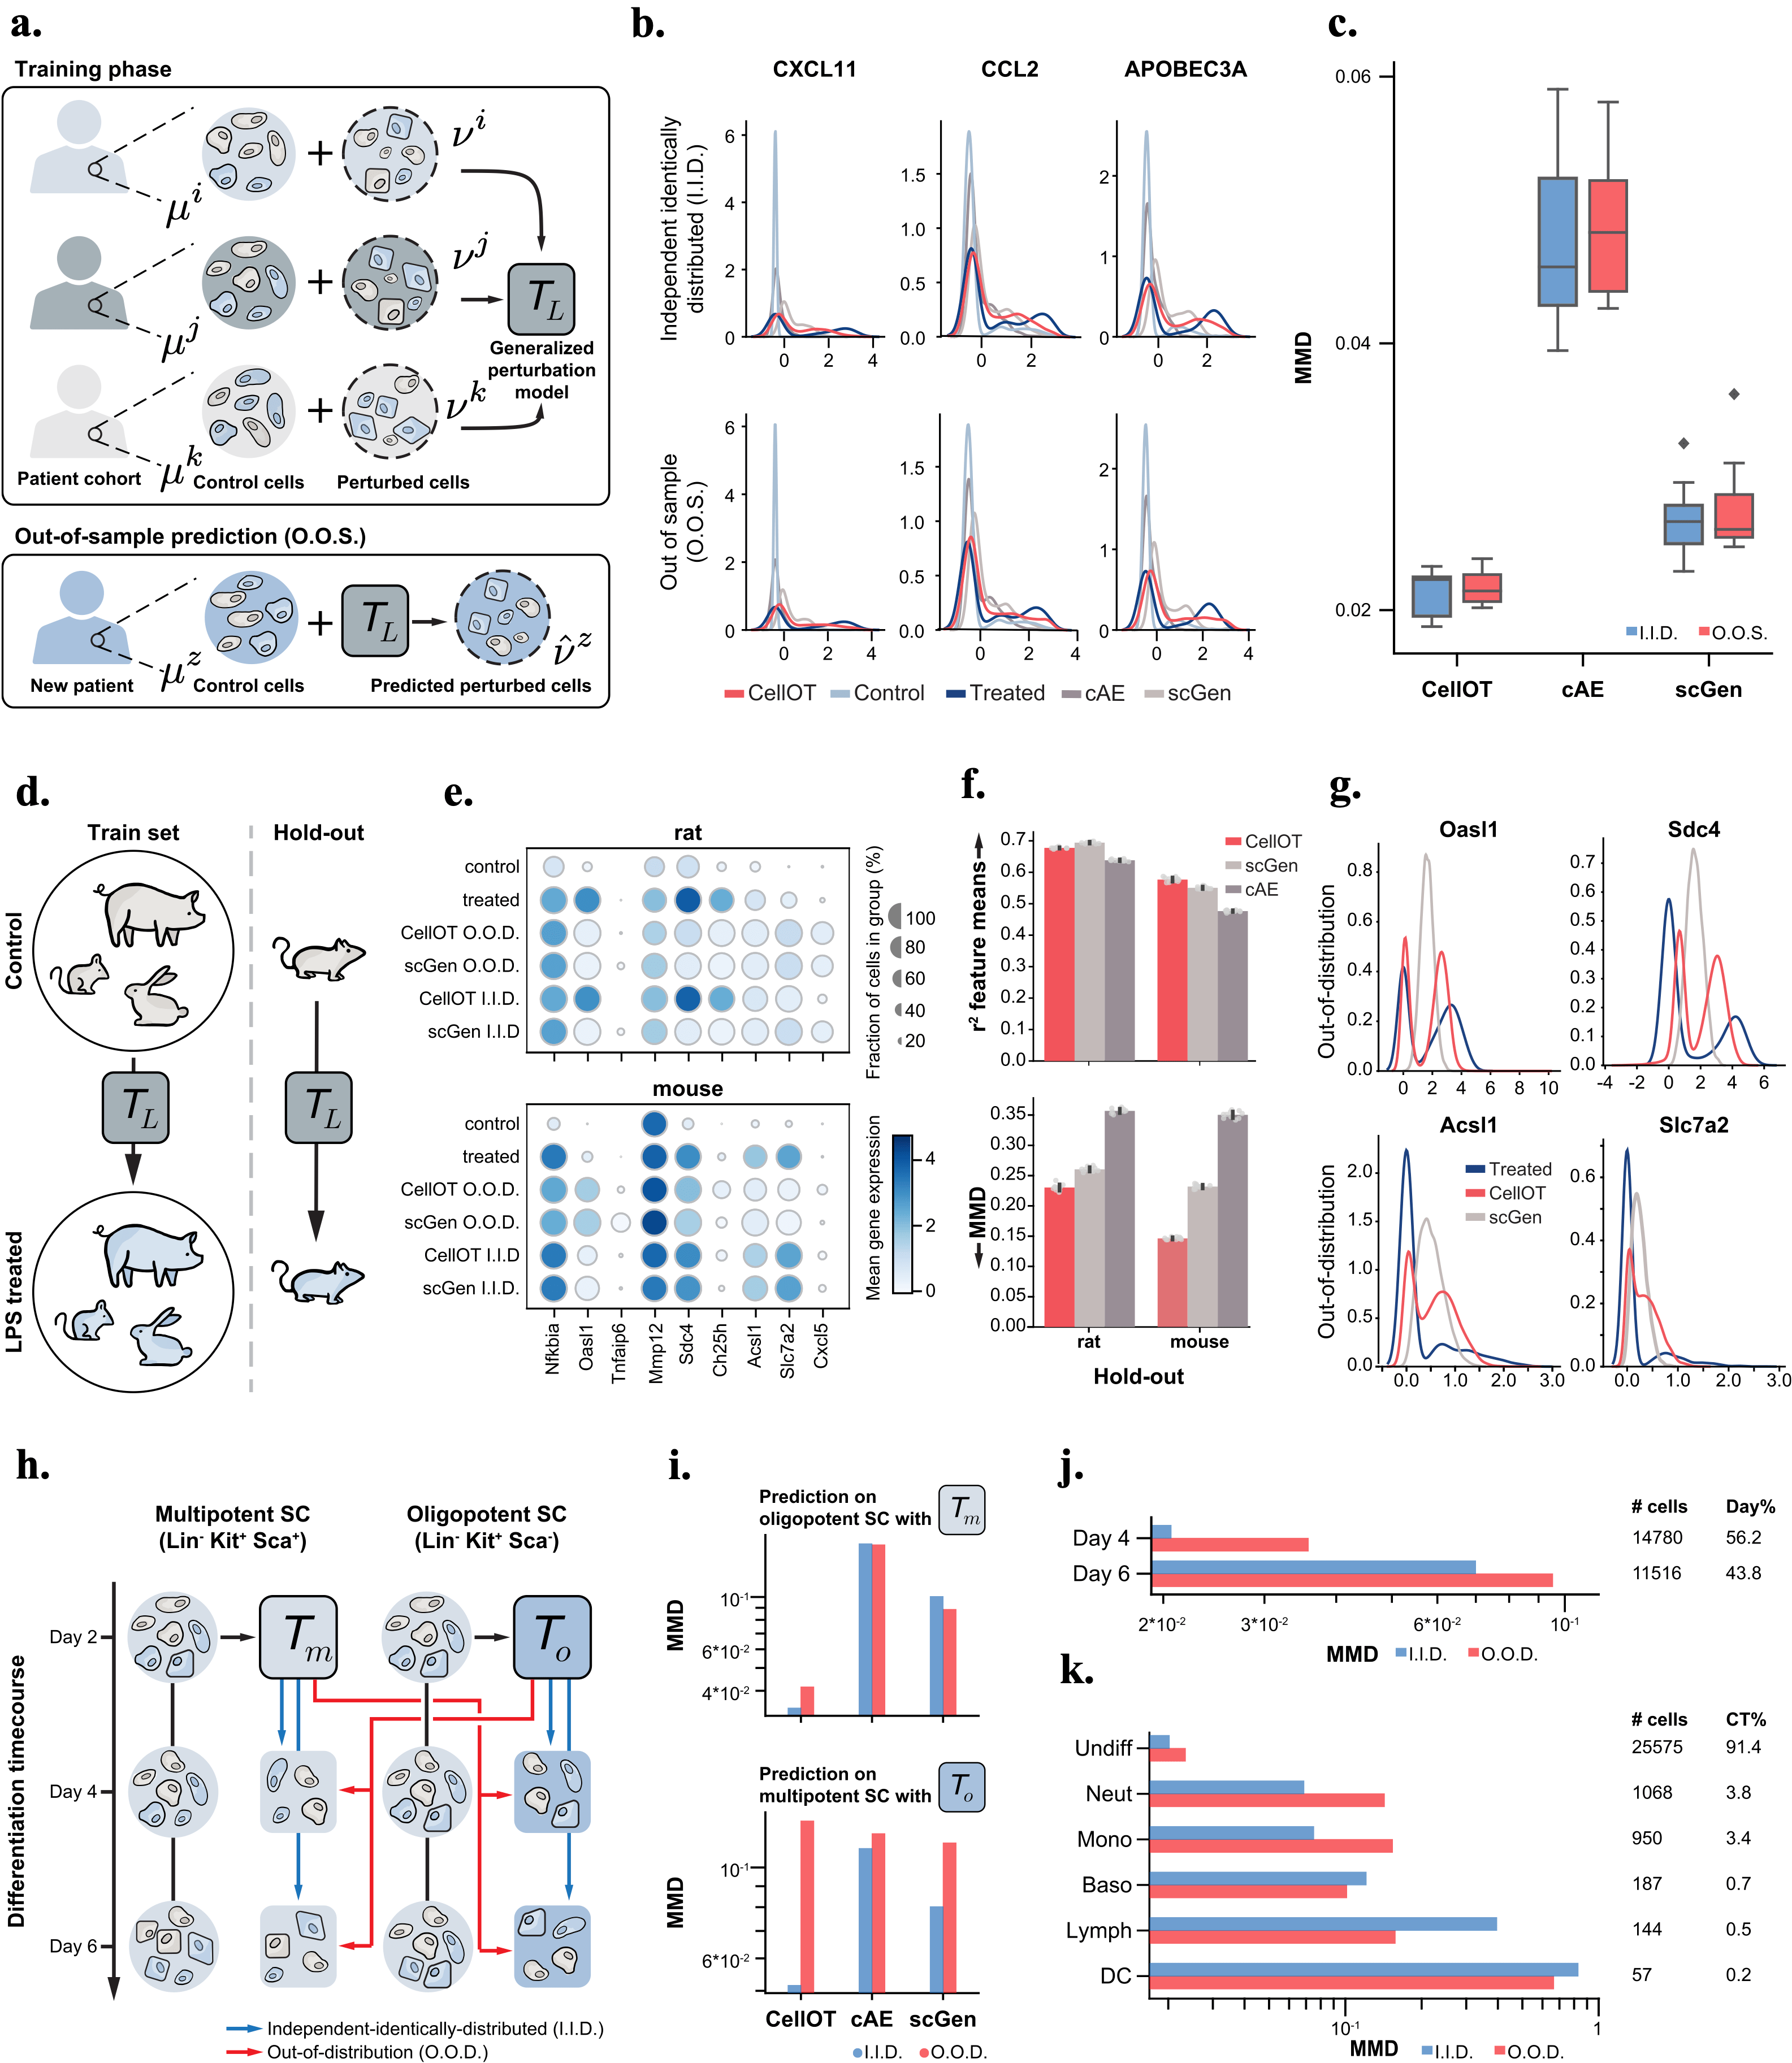
\includegraphics[width=1.05\textwidth]{figures/fig_generalization_cellot.png}
 \end{figure}
 \captionof{figure}{
    \textbf{\textsc{CellOT} generalizes to unseen patients and cell subpopulations.} Out-of-sample (o.o.s., \textbf{a-c}), and \acrlong{ood} (\acrshort{ood}, \textbf{d-k}) setting. \textbf{a.} Cells from eight lupus patients are measured in an untreated and IFN-$\beta$ treated state. 
%    For each sample, we train two models, an o.o.s.~model trained on cells from all other samples and an i.i.d.~model trained with additional access to half of the cells in the holdout sample (not shown). 
    \textbf{b.} Marginals of predicted cells from the holdout sample in the i.i.d.~(top) and o.o.s.~(bottom) setting. Predictions for both models are made on the same test set (not used for training the two models). \textbf{c.} \acrshort{MMD} scores between the predicted distribution and the observed treated distribution across all holdout samples in the i.i.d.~and o.o.s.~settings. Box plots indicate the median and quartiles.
    \textbf{d.} As an \acrshort{ood} task, we train \textsc{CellOT} and baselines to predict the response to LPS across different species, and test on rat (or mouse) as a holdout species. \textbf{e.} Mean gene expression for i.i.d. and \acrshort{ood} predictions for \textsc{CellOT} and \textsc{scGen} for selected marker genes.  \textbf{f.} Comparison of \acrshort{ood} performance for $r^2$ correlation feature means and \acrshort{MMD} of \textsc{CellOT} and baselines. Data are depicted as the mean +/- standard deviation across n=10 bootstraps of the test set. \textbf{g.} Marginals of the \acrshort{ood} predictions for marker genes showing bimodal expression profiles when using rat as a holdout.
    \textbf{h.} We apply \textsc{CellOT} to predict how cells from day 2 develop into the combined set of day 4 and 6 when trained on only multipotent cells ($T_m$) or oligopotent cells ($T_o$). We then apply $T_m$ to predict the \acrshort{ood}~oligopotent cells and $T_o$ to predict the \acrshort{ood}~multipotent cells. \textbf{i.} \acrshort{MMD} scores between the predicted and (observed) developed distributions for all models in both \acrshort{ood}~ and i.i.d.~prediction tasks (jointly for day 4 and 6). Performance of \textsc{CellOT}, when predicting \textbf{j.} day 4 states and day 6 states \textbf{k.} for different cell types in each setting using $T_m$. \vspace{10pt}}
    \label{fig:generalization_cellot}

\subsection{Reconstructing Innate Immune Responses across Different Species}
%\subsection{\textsc{CellOT} reconstructs innate immune responses across species}

The innate immune response is a cell-intrinsic defense program showing high levels of heterogeneity among responding cells and thus an ideal task for evaluating \textsc{CellOT}'s capabilities. We rely our analysis on the dataset collected by \citet{hagai2018gene}, which studies the evolution of innate immunity programs of mononuclear phagocytes within different species, including pigs, rabbits, mice, and rats. For this, these primary bone marrow-derived cells are stimulated using \acrshort{LPS}.
In the following, we test how well \textsc{CellOT} and the baselines reconstruct innate immune responses within species that are not encountered during training. We refer to the generalization task as \acrfull{ood}, since unlike the o.o.s.~setting, we expect different species to have very distinct responses (see \cref{fig:generalization_cellot}d).
The holdout set thereby consists of cells derived from either rat or mouse. See \cref{fig:crossspecies_ood_analysis}a,b for an analysis of cross-species similarity and the reasoning behind selecting the holdout set.

Indeed, \textsc{CellOT} accurately reconstructs the innate immune response in both mouse and rat in the i.i.d. and \acrshort{ood} setting. This not only becomes evident through capturing more precisely the mean expression level of marker genes that show high differential expression levels upon addition of \acrshort{LPS}, e.g., \textit{Nfkb1} (NF-$\kappa$B), \textit{Oasl1} (Oasl1), \textit{Mmp12}, and \textit{Cxcl5} (see Figs.~\ref{fig:generalization_cellot}e and \ref{fig:crossspecies_ood_analysis}c-d), but also through the average correlation coefficient $r^2$ computed between \acrshort{ood} predictions and holdout observations across all genes (see \cref{fig:generalization_cellot}f).
In particular, \textsc{CellOT} outperforms the baselines when analyzing how well each method captures the heterogeneity of innate immune responses in different species, as demonstrated by low levels of \acrshort{MMD} (see \cref{fig:generalization_cellot}f).
Most impressively, our method shows a strong alignment or gene expression marginals of aforementioned marker genes that show complicated bimodal expression profiles upon perturbation (see \cref{fig:generalization_cellot}g).

% \subsection*{\textsc{CellOT} generalizes perturbation responses \acrlong{ood} from multipotent populations to cells of lower potency}
\subsection{Generalizing Developmental Fate Decisions from Multipotent to Oligopotent Cell Populations}

\looseness -1 During developmental processes, stem and progenitor cells progress through a hierarchy of fate decisions, marked by a continuous differentiation of cells that refine their identity until reaching a functional end state.
% Modern high-throughput methods allow us to monitor these successive changes in gene expression profiles by observing multiple snapshots over time. To ultimately associate molecular differences among progenitor cells with their capacity to generate mature cell types and get a better understanding of biological differentiation or reprogramming mechanisms, we are required to learn the alignment of progenitor to mature cell states.
By tracking an initial cell population along the differentiation process, \textsc{CellOT} allows us to recover individual molecular cell fate decisions and developmental trajectories. 
% Here, the perturbation of the control population of progenitor cells is initiated by internal molecular factors driving developmental processes instead of some external factor. 

% \citet{weinreb2020lineage} use the mouse hematopoietic system as a model for a developmental process. To be able to clonally trace transcriptomes over time and capture not only each transcriptional cell state but also fate, each cell contains a genetic barcode that remains throughout cell division. This not only allows one to detect sister cells in the earliest stages of the developmental process but also links differentiated cells sampled at a later stage of the differentiation process to the original cell by reading out the barcode.

\citet{weinreb2020lineage} analyzed the fate potential of \acrfull{HSPC}, by tracking a broad class of oligopotent %(LIN$^{-}$KIT$^{+}$SCA$^{-}$) 
and multipotent %(LIN$^{-}$KIT$^{+}$SCA$^{+}$)
 progenitor cell subpopulations and observing samples on days 2, 4, and 6 (\cref{fig:generalization_cellot}h).
Here, we test how well \textsc{CellOT} and other baselines can learn the differentiation process of the cells observed on day 2 to the cells observed on days 4 and 6 (combined) and generalize from one subpopulation to another (\acrshort{ood} setting).
% Similar to the o.o.s. setting, we train two models per subpopulation.
We learn two maps, where map $T_o$ is trained exclusively on oligopotent cells, and $T_m$ on multipotent cells.
I.i.d.~versions of these maps are trained on both oligopotent and multipotent cells, such that each pair of i.i.d.~and \acrshort{ood}~maps is evaluated on the same test set.
Comparing the distributional distance between predicted and observed differentiated cell states using the \acrshort{MMD} metric, \textsc{CellOT} outperforms current state-of-the-art methods in this i.i.d.~setting for both the oligopotent and the multipotent subsets (see \cref{fig:generalization_cellot}i).
Furthermore, while baselines struggle to perform in either \acrshort{ood}~setting, \textsc{CellOT} is able to generalize its predictions in one direction, i.e., from multipotent cells to the oligopotent setting.
In contrast to oligopotent cells, multipotent cells have a higher potency and thus can potentially differentiate into more cell types, and so we would expect $T_m$ is more likely to generalize than $T_o$, trained on the less potent oligopotent cells.
When predicting developmental perturbations on multipotent cells using $T_o$, the differentiated cell fates cannot be recovered.
% For this task, the overall performance of other chosen baselines is low and equivalent to a random shift. Here, both cAE \citep{lopez2018scvi} and scGen \citep{lotfollahi2019scgen} simply predict a random shift without biological meaning.
% , at a level at which the \acrshort{MMD} metric is no longer sensitive.

\looseness -1 
% Depending on shared or individual receptors, signaling pathways, and regulatory networks, the response to perturbations and sensitivity to developmental factors or drugs might vary strongly between cell types or at different points in time.
% However, a robust perturbation model is required to capture the perturbation response across different cell types as well as at various levels of temporal resolutions.
We further compare the performance at different time points and across cell types.
% The transportation maps $T_o$ and $T_m$ were trained to learn the response from day 2 cells to day 4 and 6 together (\cref{fig:generalization_cellot}h). 
\cref{fig:generalization_cellot}j shows the accuracy of the modeled development of multipotent cells using map $T_m$ individually for day 4 and day 6 cells, respectively. It is evident that \textsc{CellOT} achieves better results when predicting developmental dynamics short-range instead of states further away in time.
This suggests a potential limitation for all of these methods, which might be unable to recover alignments over coarse time resolutions.
% In addition, we further decompose the analysis to capture \textsc{CellOT}'s consistency across different cell types. 
Beyond, while the vast majority of cells on days 4 and 6 are still undifferentiated (undiff), some cells have evolved into neutrophils (neut), monocytes (mono), basophils (baso), lymphoid precursors (lymph), or dendritic cells (DC).
As expected, the performance of \textsc{CellOT} drops in terms of the \acrshort{MMD} metric for those cell types that are only sparsely represented in the dataset (see \cref{fig:generalization_cellot}k).

\section{Discussion}

Single-cell expression profiling provides a detailed look into the molecular states of individual cells, but it is destructive and does thus not allow continuous measurements of molecular properties over time. There have been numerous proposals for methods to uncover the dynamics of individual cells from population data, but all of them face the same challenge: sequentially observed distribution of cell states can be produced by multiple dynamics and mechanisms of gene regulation. The ill-defined nature of the problem makes it necessary to pose certain assumptions on the underlying cellular dynamics.

The mathematical foundation of this work builds on the biological intuition that perturbations incrementally alter the molecular profiles of cells. This principle aligns with the theory of optimal transport and, following previous work \citep{schiebinger2019optimal}, serves naturally as the model foundation of \textsc{CellOT}.
If this principle is violated, however, and perturbations strongly disrupt the population to an unidentifiable level, the performance of \textsc{CellOT} as well as other methods drops (see Discussion).
In these instances, more complicated mathematical machinery would be needed.
Such tools, however, are currently unable to scale to settings with more than a few genes \citep{heydari2022iqcell}.
Thus, we rely on a fine granularity of the time course to recover large cell state changes between consecutive time points \citep{tritschler2019concepts}.

Furthermore, if a system exhibits rotations and oscillations within two consecutive snapshots not captured by measurements, models based on optimal transport and previous tools \citep{weinreb2018fundamental} will not be able to recover such complex dynamics. This is in part also due to the current choice of the cost function, which, due to theoretical constraints and practical performance, is set to the Euclidean distance. We leave it to future work, to investigate choices of alternative cost functions. 

Beyond, the current system is not able to recover effects (other than cell flux) that change the distribution of cells between time points, for example, proliferation and death \citep{tritschler2019concepts}. Recent works propose extensions to the classical neural optimal transport scheme that account for cell death and birth \citep{lubeck2022neural}.

Lastly, current developments in bioengineering aim at overcoming the technological limitation of destructive cell assays. \citet{chen2022live} propose a transcriptome profiling approach that preserves cell viability. \citet{weinreb2020lineage} capture cell differentiation processes while clonally connecting cells and their progenitors through barcodes. These methods thus offer (lower-throughput) insights that provide individual trajectories of cells over time, i.e., an alignment between distinct measurement snapshots.
\citet{somnath2023aligned} propose a novel algorithmic framework connected to optimal transport that is able to make use of such (partially) aligned datasets \citep{shi2023diffusion, tong2023conditional}. 
